\documentclass[12pt]{ctexart}
\usepackage{amsmath,graphicx,textcomp,subfigure,indentfirst,ctex,color,float}
\usepackage{bm, mhchem}
\title{Lecture 10}
\author{赵思逸}

\date{\today}
\newcommand{\new}[1]{\textcolor{blue}{#1}}

\newcommand{\refeq}[1]{式~(\ref{#1})}
\newcommand{\reffig}[1]{图~(\ref{#1})}

\begin{document}

\maketitle
\new{
极早期宇宙的热历史
\begin{itemize}
    \item 再复合 发生在 $T \sim 0.3 \mathrm{~eV}$.
    \item \ce{^{4}He} 退耦 发生在 $T \sim 0.07 \mathrm{~MeV}$.
    \item 中子退耦 发生在 $T \sim 0.5 \mathrm{~MeV}$.
    \item 中微子退耦 发生在 $T \sim 1 \mathrm{~MeV}$.
\end{itemize}
}
% \begin{itemize}
%     \item 从宇宙的诞生到中微子退耦,宇宙处于热平衡状态,温度 $T \sim 10^9 \mathrm{~K}$.
%     \item 再复合后,宇宙处于非热平衡状态,温度 $T \sim 10^4 \mathrm{~K}$.
%     \item He4 退耦后,宇宙处于热平衡状态,温度 $T \sim 10^4 \mathrm{~K}$.
%     \item 中子退耦后,宇宙处于热平衡状态,温度 $T \sim 10^4 \mathrm{~K}$.
%     \item 中微子退耦 $T \sim 1 \mathrm{~MeV}$ 后,宇宙处于热平衡状态,温度 $T \sim 1 \mathrm{~MeV}$.
% \end{itemize}

\section{中微子退耦(neutrino decoupling)}

中微子退耦发生在约 $1 \mathrm{~MeV}$ 时。

在$T> 10 \mathrm{~MeV}$时,正负电子和正负中微子通过弱相互作用 $e^+ + e^- \leftrightarrow \nu + \bar{\nu}$ 互相转化达到热平衡,康普顿散射使电子和光子达到热平衡。此时质子、中子、电子、光子、中微子都处于热平衡之中。

当 $T \sim 1 \mathrm{~MeV}$ 时,弱相互作用的反应不够有效,中微子退耦。此时质子、中子、电子、光子处于热平衡之中。

当 $T \sim 0.5 \mathrm{~MeV}$ 时,即约为电子的静质量时,电子变成非相对论性粒子,将部分能量转移给光子,导致光子温度上升。而此时中微子已经退耦,自行绝热膨胀,不会接收这部分能量,导致光子温度大于中微子。质子和中子比电子重很多,此时为非相对论粒子,虽然也处在热平衡中,但能量贡献不变,以下计算能量转移不考虑质子和中子。

以下计算光子(微波背景辐射)温度比中微子(背景辐射)温度高多少。

定义熵密度 $s(T) = \frac{\rho+P}{T}$,热平衡系统$s\propto a^{-3}$.
粒子数密度为(假设化学势为0)
\begin{equation}
    n(p) dp = \frac{4\pi g p^2}{h_{\mathrm{pl}}^3} \frac{1}{\exp\left(\frac{\sqrt{p^2+m^2}}{k_B T}\right) \pm 1}
\end{equation}
费米子(Fermion, 如电子、中微子)取正号,玻色子(Boson, 如光子)取负号。

能量密度
\begin{equation}
    \rho (T) = \int_0^\infty n(p,T) dp \sqrt{p^2+m^2}
\end{equation}

相对论性粒子
\begin{equation}
    \rho(T) =
    \begin{cases}
        \frac{1}{2} g a_B T^4   & \text{Boson} \\ 
        \frac{7}{8} \times \frac{1}{2} g a_B T^4 & \text{Fermion}
    \end{cases}
\end{equation}
其中$g$是粒子的简并度,包括粒子种类(比如中微子有三代)、正反粒子、自旋态。$a_B$是常数。
记为 $\rho(T) = \frac{1}{2} \mathcal{N} a_B T^4 $, 则
\begin{equation}
    \mathcal{N} =
    \begin{cases}
        g  & \text{Boson} \\ 
        \frac{7}{8} \times g  & \text{Fermion}
    \end{cases}
\end{equation}

对相对论性粒子,$P=\frac{1}{3}\rho$.
代入熵密度定义得到
$s(T) = \frac{4\rho}{3T} = \frac{2}{3} \mathcal{N} a_B T^3$,
由于$s(T) a^3 = const.$,
所以 
$\mathcal{N} a^3 T^3 = const.$

中微子退耦时间$t_\text{dec}$,此时温度 $T_\nu(t_\text{dec}) = T_\gamma(t_\text{dec}) = T_\text{dec}$.

\begin{equation}
    \mathcal{N}_\text{dec} = 2+ 1\times 2\times 2\times \frac{7}{8} = \frac{11}{2}
\end{equation}
其中第一项来自光子,第二项来自电子,其中1、2、2分别对应电子的种类、正反粒子、两个自旋态。

当 $t_* \gg t_\text{dec}$, 电子变成非相对论性粒子,不再考虑,所以
\begin{equation}
    \mathcal{N}(t_*) = 2
\end{equation}

中微子退耦后,自行按照 $T_\nu \propto \frac{1}{a}$ 演化,不受 $\mathcal{N}$ 变化的影响,所以
$T_\text{dec} a_\text{dec} = T_\nu (t_\text{dec}) a_\text{dec} = T_\nu(t_*) a(t_*)$.
由于光子和电子共同处于热平衡,所以 
\begin{equation}
    \mathcal{N}_\text{dec} a_\text{dec}^3 T_\text{dec}^3 = \mathcal{N}(t_*) a^3(t_*) T_\gamma^3(t_*)
\end{equation}
可以得到
\begin{equation}
    \frac{T_\nu(t_*)}{T_\gamma(t_*)} = \left(\frac{\mathcal{N}(t_*)}{\mathcal{N}_\text{dec}}\right)^\frac{1}{3} = \left(\frac{4}{11}\right)^\frac{1}{3} \simeq \frac{1}{1.4} 
\end{equation}

此后,光子和中微子都按照 $T\propto \frac{1}{a}$ 各自演化,可得今天
\begin{equation}
    \frac{T_{\nu,0}}{T_{\gamma,0}} = \frac{T_\nu(t_*)}{T_\gamma(t_*)} = \frac{1}{1.4}
\end{equation}

上面说的光子到今天红移到微波波段,即CMB。我们测量得到CMB的温度 $T_{\gamma,0}\simeq 2.725 \mathrm{~K}$, 则可推知中微子背景辐射 C$\nu$B 的温度$T_{\nu,0} \simeq 1.945 \mathrm{~K}$.

宇宙辐射能量密度
\begin{equation}
    \rho_{R,0} = \rho_{\gamma,0} + \rho_{\nu,0} = \frac{1}{2} a_B T_{\gamma,0}^4 \left(2+ 3\times 2\times 1\times\frac{7}{8} \times \left(\frac{4}{11}\right)^\frac{4}{3} \right) = 1.681 \rho_{\gamma,0}
\end{equation}
其中括号内第一项是光子,第二项是中微子,其中3、2、1分别对应中微子有三代(电子中微子$\nu_e$、缪子中微子$\nu_\mu$、陶子中微子$\nu_\tau$)、正反中微子、正反中微子各对应一个自旋态,7/8是由于中微子是费米子,$\left(\frac{4}{11}\right)^\frac{1}{3}$是中微子和光子的温度比,另外它的四次方因为能量密度正比于温度的4次方。

\section{暴涨理论(Inflation Theory)}

大爆炸理论中存在三个重要的疑难。

\subsection{平坦性问题(Flatness Problem)}
考虑物质主导的非平坦宇宙,
\begin{equation}
    \rho_m(t) = \Omega_M \rho_\text{crit} \left( \frac{a}{a_0}\right)^{-3}
\end{equation}

\begin{equation}
    |\Omega(t)-1| = \left|1+\frac{\Omega_M a_0}{\Omega_K a}\right|^{-1}
\end{equation}
%

假设 $\Omega_M = 0.9$, $\Omega_K = 0.1$, 
在 CMB 时期,$z=1000,  |\Omega(t)-1|  \simeq 10^{-4}$,
在 BBN 时期,$ |\Omega(t)-1|  \simeq  10^{-12}$.

可见即使今天的 $\Omega_K$ 不是很小,在宇宙早期  $\Omega_K$ 也是非常小的,这是需要解释的。

\subsection{视界疑难(Horizon Problem)}

CMB在全天$4\pi$立体角都高度各向同性,而CMB时期的粒子视界是有限大的。
\begin{equation}
    d_H (t_\text{CMB}) \simeq \frac{cH_0^{-1}}{\Omega_M^\frac{1}{2}\left(1+z_\text{CMB}\right)^\frac{3}{2} } \simeq 0.015 \mathrm{~rad} \sqrt{\Omega_M} \simeq 1^\circ 
\end{equation}
对应今天天空中的$1^\circ $, 天空中间隔超过$1^\circ $的两点在CMB时期并没有因果联系,它们的温度接近并不自然。

\subsection{磁单极子问题(Magnetic monopole)}

大统一理论(GUT)预言了磁单极子的存在,并且预言了较高的磁单极子密度。但是人们并没有观测到磁单极子。这个问题正是Alan Guth等人提出暴涨理论的动机。

\subsection{种子涨落的起源}

CMB的微小各向异性很难用热涨落解释,需要其它的起源。

\subsection{暴涨理论}

1981年,Alan Guth等人提出了暴涨理论。
暴涨理论认为宇宙极早期出现过一段指数膨胀的时期,$a\propto e^{Ht}$,在很短的时间内,宇宙膨胀了$e^{60}$倍,同时有某种物理机制使得暴涨结束。

\begin{itemize}
    \item 平坦性问题:暴涨前的宇宙可能有曲率,但暴涨使得我们今天的宇宙来自其中的一小块,所以很平坦。
    \item 视界疑难:暴涨后到CMB之间,辐射占主导,视界逐渐增大,但在暴涨时期,视界曾经随时间变小。原本有因果联系的两点退出彼此的视界,成为CMB上“没有因果联系”的两点,因此在暴涨后它们的温度仍然高度相同,如同处于热平衡。
    \item 磁单极子问题:暴涨使得磁单极子彼此急剧远离,导致今天的视界内平均不到一个磁单极子。
    \item 种子涨落的起源:暴涨使得微观上的量子涨落在短时间内被拉到宇宙的尺度上,成为经典的密度涨落。
\end{itemize}

\subsubsection*{如何实现暴涨?}

Alan Guth等人在1981年提出的简单模型:暴涨子在假真空态上提供相当于暗能量的效应,使宇宙加速膨胀,当暴涨子发生量子隧穿到达真的真空态上,暴涨结束。但是这样得出的种子涨落太大。如 \reffig{suichuan} 。

1982-1983年,Andrei Linde 改进提出慢滚模型(slow-roll),该模型中暴涨子在一个较平的假真空上缓慢滚动,当滚到真的真空态上时结束暴涨。如  \reffig{slow-roll} 。

慢滚模型是目前人们较为普遍接受的一种最简单的模型,但慢滚模型预言的原初引力波目前还没有观测到,因此有很多其它的暴涨模型,有待未来的观测告诉我们更多的信息。

\begin{figure}[!hbtp]
	\centering
	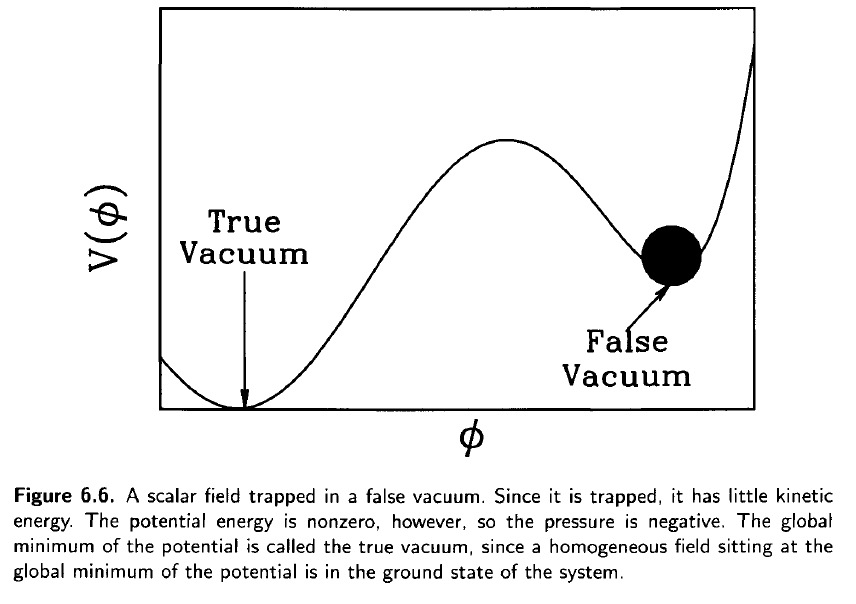
\includegraphics[width=1.0\linewidth]{suichuan.jpg}
	\caption{引自S. Dodelson.} \label{suichuan}
\end{figure}

\begin{figure}[!hbtp]
	\centering
	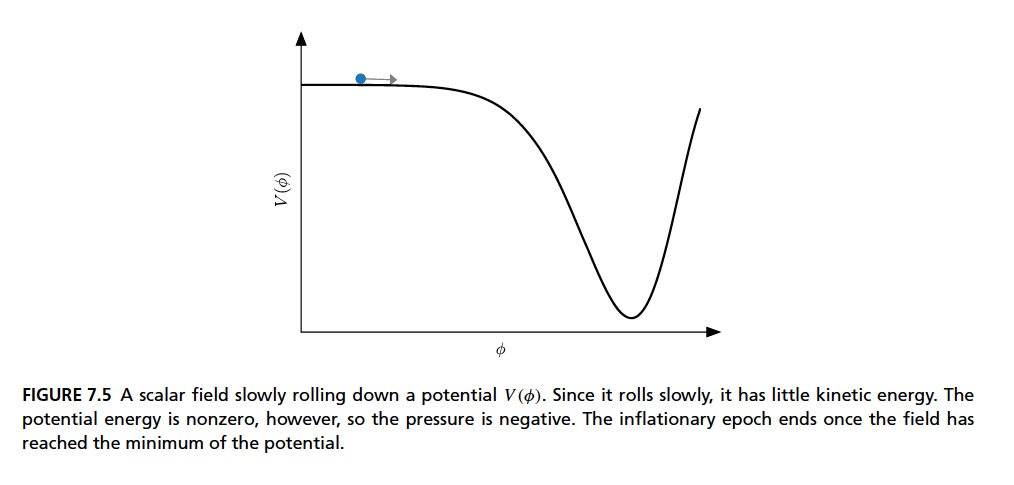
\includegraphics[width=1.0\linewidth]{slow-roll.jpg}
	\caption{引自 S. Dodelson \& F. Schmidt (second edition)} \label{slow-roll}
\end{figure}

\end{document}
